\documentclass[crop,tikz]{standalone}

\usepackage{amsmath}

\begin{document}

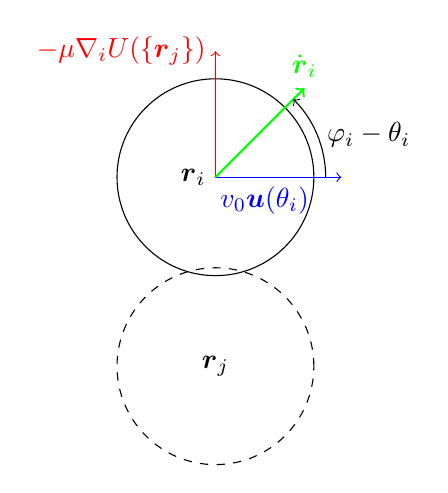
\begin{tikzpicture}
\draw[dashed] (0, 0) node{$\boldsymbol{r}_j$} circle (1.25);
\draw (0, 2.4) node[left]{$\boldsymbol{r}_i$} circle (1.25);
\draw[red, ->] (0, 2.4) -- (0, 4) node[left]{$-\mu \nabla_i U(\{\boldsymbol{r}_j\})$};
\draw[blue, ->] (0, 2.4) -- (1.6, 2.4) node[midway, below]{$v_0 \boldsymbol{u}(\theta_i)~~~$};
\draw[green, thick, ->] (0, 2.4) -- ({0 + cos(45)*1.6}, {2.4 + sin(45)*1.6}) node[above]{$\dot{\boldsymbol{r}}_i$};
\draw[->] (1.4, 2.4) arc (0:45:1.4) node[midway, right]{$\varphi_i - \theta_i$};
\end{tikzpicture}

\end{document}
